% !TEX root = knottedMain.tex
\documentclass[varwidth=\maxdimen]{standalone}

\usepackage{mathtools,amssymb,mathrsfs,dutchcal,upgreek,faktor,accents,etoolbox,multicol}
\usepackage[dvipsnames]{xcolor}
\definecolor{mygreen}{RGB}{	8,156,79 }
\usepackage{tikz,tikz-cd}
\usetikzlibrary{patterns,knots,arrows.meta,decorations.markings}
\tikzset{>={Straight Barb[scale=0.85]}}
\tikzcdset{
  cells={font=\everymath\expandafter{\the\everymath\displaystyle}},
  arrow style=tikz,
  diagrams={>={Straight Barb[scale=0.85]}},
  every label/.append style = {font = \small}
}

\newcommand{\deriv}{\mathcal{D}}
\newcommand{\const}{\mathsf{const}}
\newcommand{\refl}{\mathsf{refl}}


\begin{document}
\begin{tikzcd}[column sep=large]
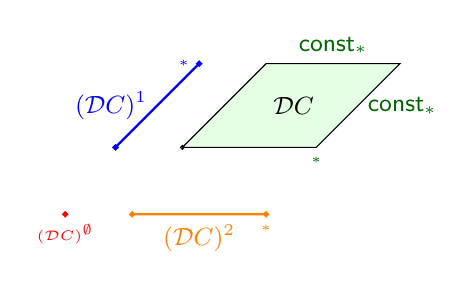
\begin{tikzpicture}[scale=0.85,font=\small]
    \fill[red,thick,draw=red]
        (-1.25,-0.5) circle (0.8pt) node[below]{\tiny$(\deriv C)^\emptyset$};
    \fill[blue,thick,draw=blue]
        (-0.5,0.5) circle (0.8pt) %node[left]{\tiny$r^1(\deriv A)^\emptyset$}
        -- (0.75,1.75) circle (0.8pt) node[pos=0.5, left]{$(\deriv C)^1$} node[left]{\tiny$*$};
    \fill[orange,thick,draw=orange]
        (-0.25,-0.5) circle (0.8pt) %node[below]{\tiny$r^2(\deriv A)^\emptyset$}
        -- (1.75,-0.5) circle (0.8pt) node[pos=0.5, below]{$(\deriv C)^2$} node[below]{\tiny$*$};
    \draw[fill=green!10!white,text=green!40!black]
        (0.5,0.5) circle (0.8pt) %node[below]{\tiny$rr(\deriv A)^\emptyset$}
        -- (2.5,0.5) %node[pos=0.5, below]{\scriptsize$r^1(\deriv A)^2$} circle (0.8pt) 
        node[below]{\tiny$*$}
        -- (3.75,1.75) node[pos=0.5,right]{$\const_*$}
        -- (1.75,1.75) node[pos=0.5, above]{$\const_*$}
        -- (0.5,0.5) %node[pos=0.5,left]{\scriptsize$r^2(\deriv A)^1$} 
        node[pos=0.5, right=0.5cm, black]{$\deriv C$};
\end{tikzpicture}
    \arrow[|->]{r}{\chi} &\quad
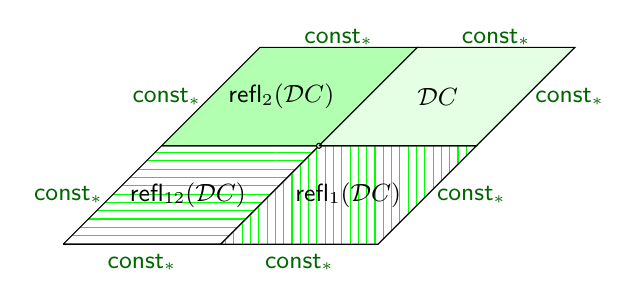
\begin{tikzpicture}[font=\small]
    \clip (-3.2,-1.15) rectangle (4.1,2);
    % front rombs
    \draw[pattern=horizontal lines, pattern color= green,text=green!40!black]
        (-2.75,-0.75)
        -- (-0.75,-0.75) node[pos=0.5, below]{$\const_*$}
        -- (0.5,0.5)
        -- (-1.5,0.5)
        -- (-2.75,-0.75) node[pos=0.5,left]{$\const_*$} node[pos=0.5, right=0.1cm, black]{$\refl_{12}(\deriv C)$};
    \draw[pattern=vertical lines, pattern color= green,text=green!40!black]
        (-0.75,-0.75)
        -- (1.25,-0.75) node[pos=0.5, below]{$\const_*$}
        -- (2.5,0.5) node[pos=0.5,right]{$\const_*$}
        -- (0.5,0.5)
        -- (-0.75,-0.75) %node[pos=0.8]{\tiny$(r^2f^1)^{h^1}$} 
        node[pos=0.5, right=0.2cm, black]{$\refl_1(\deriv C)$};
    % back rombs
    \draw[fill=green!30!white, text=green!40!black]
        (-1.5,0.5)  %node[left]{\tiny$*$}
        -- (0.5,0.5) %node[pos=0.5]{\scriptsize$(r^1f^2)^{h^2}$}
        -- (1.75,1.75) %node[pos=0.5,right]{$\const_*$}
        -- (-0.25,1.75) node[pos=0.5, above=-3pt]{$\const_*$}
        -- (-1.5,0.5) node[pos=0.5,left]{$\const_*$}
        node[pos=0.5, right=0.1cm, black]{$\refl_2(\deriv C)$};
    \draw[fill=green!10!white,text=green!40!black]
        (0.5,0.5) circle (0.9pt) %node[above]{\scriptsize$rrf^\emptyset$}
        -- (2.5,0.5) %node[pos=0.5]{\scriptsize$r^1f^2$}
        -- (3.75,1.75) node[pos=0.5,right]{$\const_*$}
        -- (1.75,1.75) node[pos=0.5, above=-3pt]{$\const_*$}
        -- (0.5,0.5) %node[pos=0.5]{\footnotesize$r^2f^1$} 
        node[pos=0.5, right=0.5cm, black]{$\deriv C$};
\end{tikzpicture}
\end{tikzcd}


\end{document}